\documentclass{article}

\usepackage[a4paper, total={7in, 9in}]{geometry}
\pagestyle{empty} % Prevent relative page numbers

%%%%%%%%%%%%%%%%%%%%%%%%%%%%%%%%%%%%%%
%% Default definitions 
%% Define listings format
\usepackage{xcolor} % Required for listings color definitions
\definecolor{Brown}{cmyk}{0,0.81,1,0.60}
\definecolor{OliveGreen}{cmyk}{0.64,0,0.95,0.40}
\definecolor{CadetBlue}{cmyk}{0.62,0.57,0.23,0}
\definecolor{lightlightgray}{gray}{0.9}

\usepackage{listings} % computer code language formatting

\lstdefinestyle{tex-style} {
	language=[LaTeX]TeX,                    % Code langugage
	basicstyle=\ttfamily,                   % Code font, Examples: \footnotesize, \ttfamily
	%keywordstyle=\color{OliveGreen},        % Keywords font ('*' = uppercase)
	commentstyle=\color{gray},              % Comments font
	numbers=none,                           % Line nums position
	numberstyle=\tiny,                      % Line-numbers fonts
	stepnumber=1,                           % Step between two line-numbers
	numbersep=5pt,                          % How far are line-numbers from code
	backgroundcolor=\color{lightlightgray}, % Choose background color
	frame=single,                             % A frame around the code
	tabsize=2,                              % Default tab size
	captionpos=b,                           % Caption-position = bottom
	breaklines=true,                        % Automatic line breaking?
	breakatwhitespace=false,                % Automatic breaks only at whitespace?
	showspaces=false,                       % Dont make spaces visible
	showtabs=false,                         % Dont make tabls visible
	columns=flexible,                       % Column format
	morekeywords={__global__, __device__}  % CUDA specific keywords
}
\lstnewenvironment{latex}
{\lstset{language=[LaTeX]TeX}}
{}
\lstset{style=tex-style}

%% Define URL format
\usepackage[hyphens]{url}
\usepackage{hyperref}
\hypersetup{
	colorlinks=true,
	citecolor=black,
	filecolor=black,
	linkcolor=blue,
	urlcolor=blue
}

\setlength\parindent{0pt}


%%%%%%%%%%%%%%%%%%%%%%%%%%%%%%%%%%%%%%
%% Example-specific packages
%\usepackage{hyperref}
\usepackage{graphicx}
\usepackage[noabbrev]{cleveref}

%%%%%%%%%%%%%%%%%%%%%%%%%%%%%%%%%%%%%%
%% Example-specific preamble


\begin{document}

\section*{The \texttt{cleveref} package}

\subsection*{Description}
\verb|cleveref| is a very powerful package which provides functionality for cross-referencing within a document. See the example for an overview of the functionality.

\textbf{Warning 1}: \verb|cleveref| has to be loaded after \verb|hyperref|\\
\textbf{Warning 2}: \verb|cleveref| is not compatible with \verb|ieeetrantools| (see links below). That means that it cannot refer to \texttt{IEEEeqnarray} environments properly. Some workarounds may exist but they are not guaranteed not to break anything else.

\subsection*{Sources}
\url{http://ctan.math.utah.edu/ctan/tex-archive/macros/latex/contrib/cleveref/cleveref.pdf}\\
\url{https://tex.stackexchange.com/questions/1863/which-packages-should-be-loaded-after-hyperref-instead-of-before#1868}\\
\url{https://tex.stackexchange.com/questions/227137/how-to-use-cleveref-with-ieeeeqnarray}\\
\url{https://tex.stackexchange.com/questions/132823/ieeetrantools-clash-with-cleveref}\\
\url{https://tex.stackexchange.com/questions/250733/ieeetran-cls-and-cleveref-the-special-case-of-ieeeeqnarray}
\url{https://tex.stackexchange.com/questions/119225/cleveref-cleveref-appears-to-not-be-so-clever-sorry-for-the-pun-but-i-couldnt}

\subsection*{Used Packages}
\verb|graphicx, hyperref, cleveref|

\subsection*{Preamble}
\begin{latex}
%%%%%%%%%%%%%%%%%%%%%%%%%%%%%%%%%%%%%%
%% Example-specific packages
\usepackage{hyperref}
\usepackage{graphicx}
\usepackage[noabbrev]{cleveref}

%%%%%%%%%%%%%%%%%%%%%%%%%%%%%%%%%%%%%%
%% Example-specific preamble
\end{latex}

\subsection*{Document}
\begin{latex}
\begin{figure}[b]
	\centering
	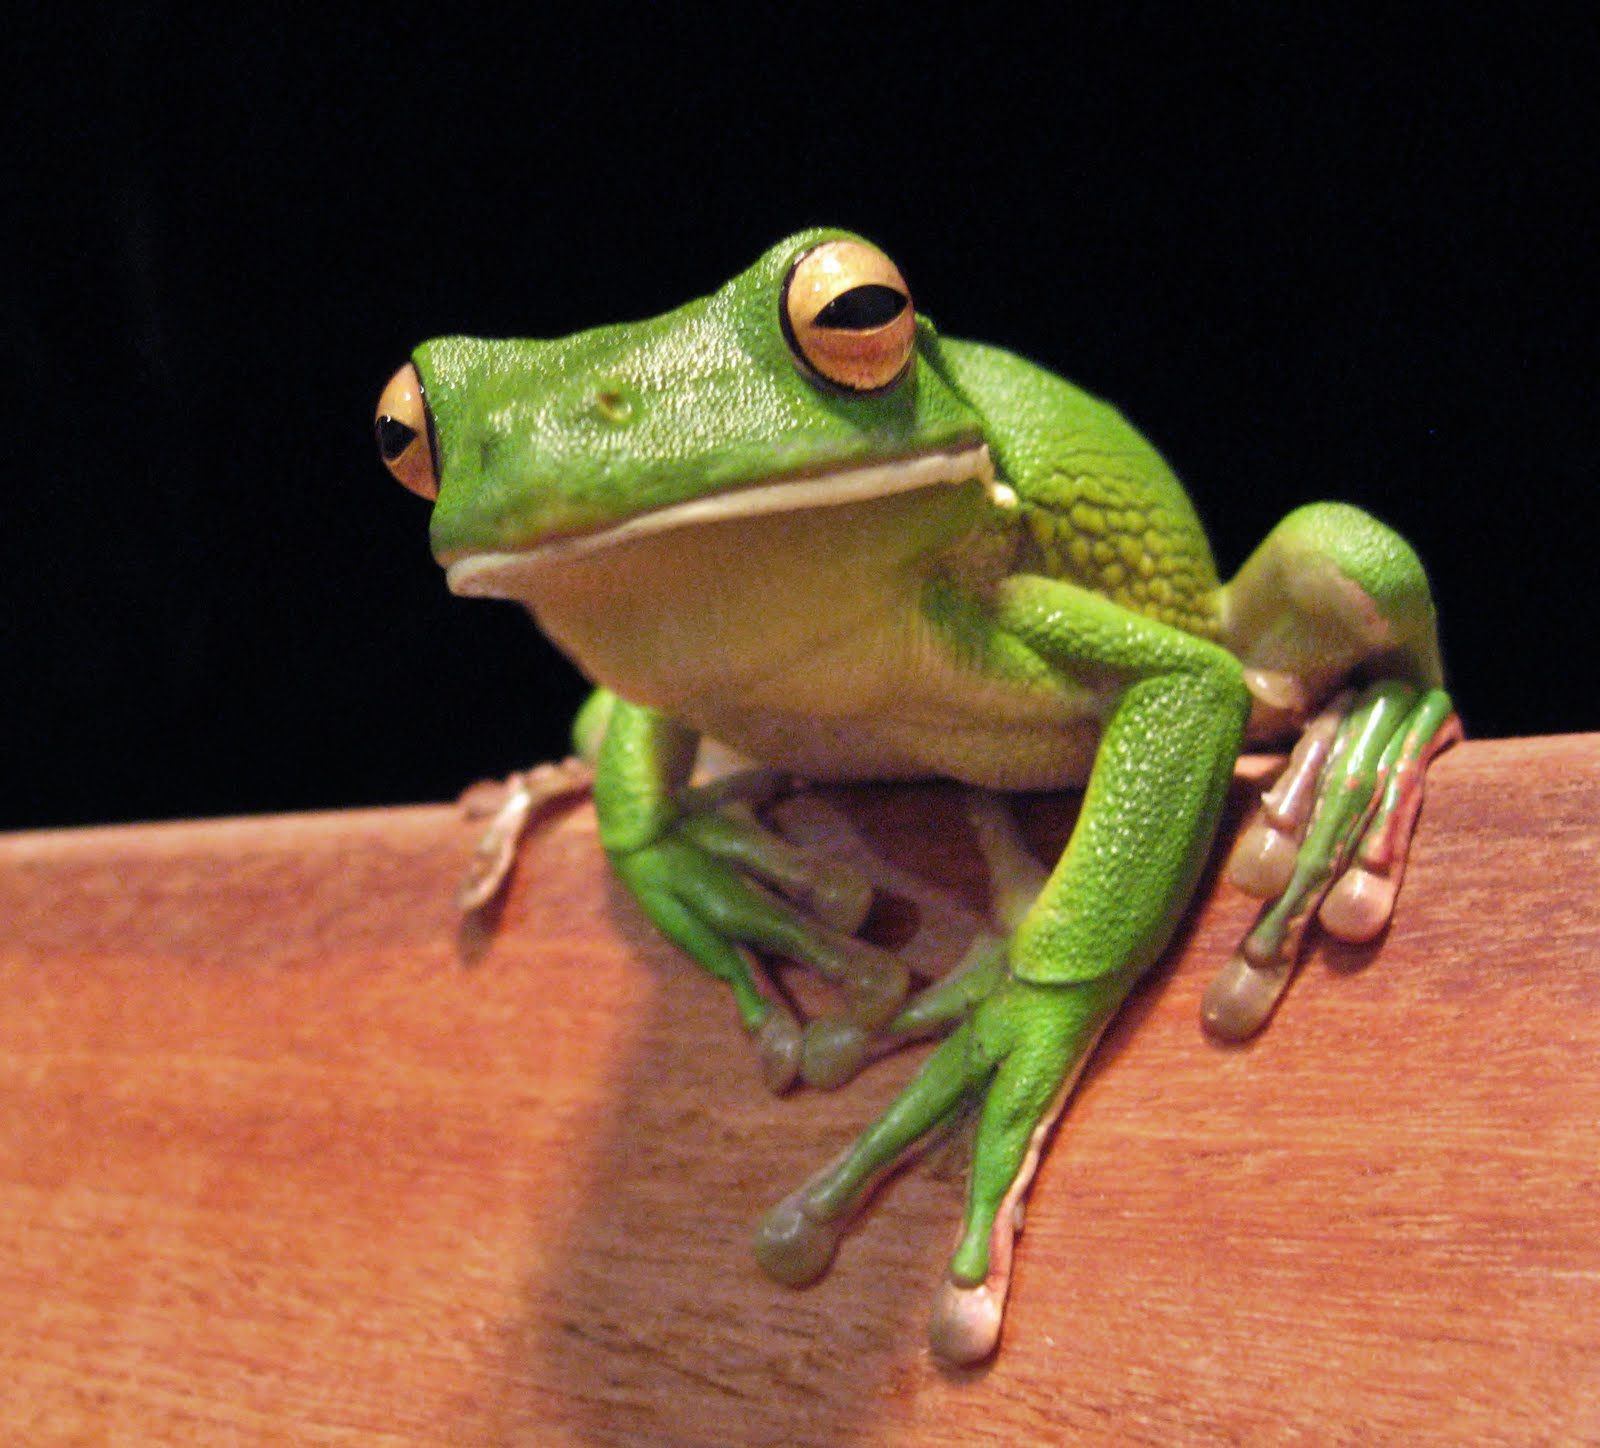
\includegraphics[width=0.25\linewidth]{frog.jpg}
	\caption{This is a figure}
	\label{fig:1}
\end{figure}

\begin{equation}
x^2+y^2=z^2
\label{eq:1}
\end{equation}
\begin{equation}
e^{\pi} = -1
\label{eq:2}
\end{equation}

The cleveref package allows you to:
\begin{itemize}
	\item prefix the type of the reference automatically: \cref{fig:1}
	\item reference with small and capital initial letters: \Cref{eq:1}, \cref{eq:1}.
	\item reference a range: \crefrange{eq:1}{eq:2}
	\item get the type of the reference: \namecref{fig:1}, \namecref{eq:1}
	\item get the page number of the reference: \cpageref{eq:1}
\end{itemize}
\end{latex}

\subsection*{Result}
\begin{figure}[h]
	\centering
	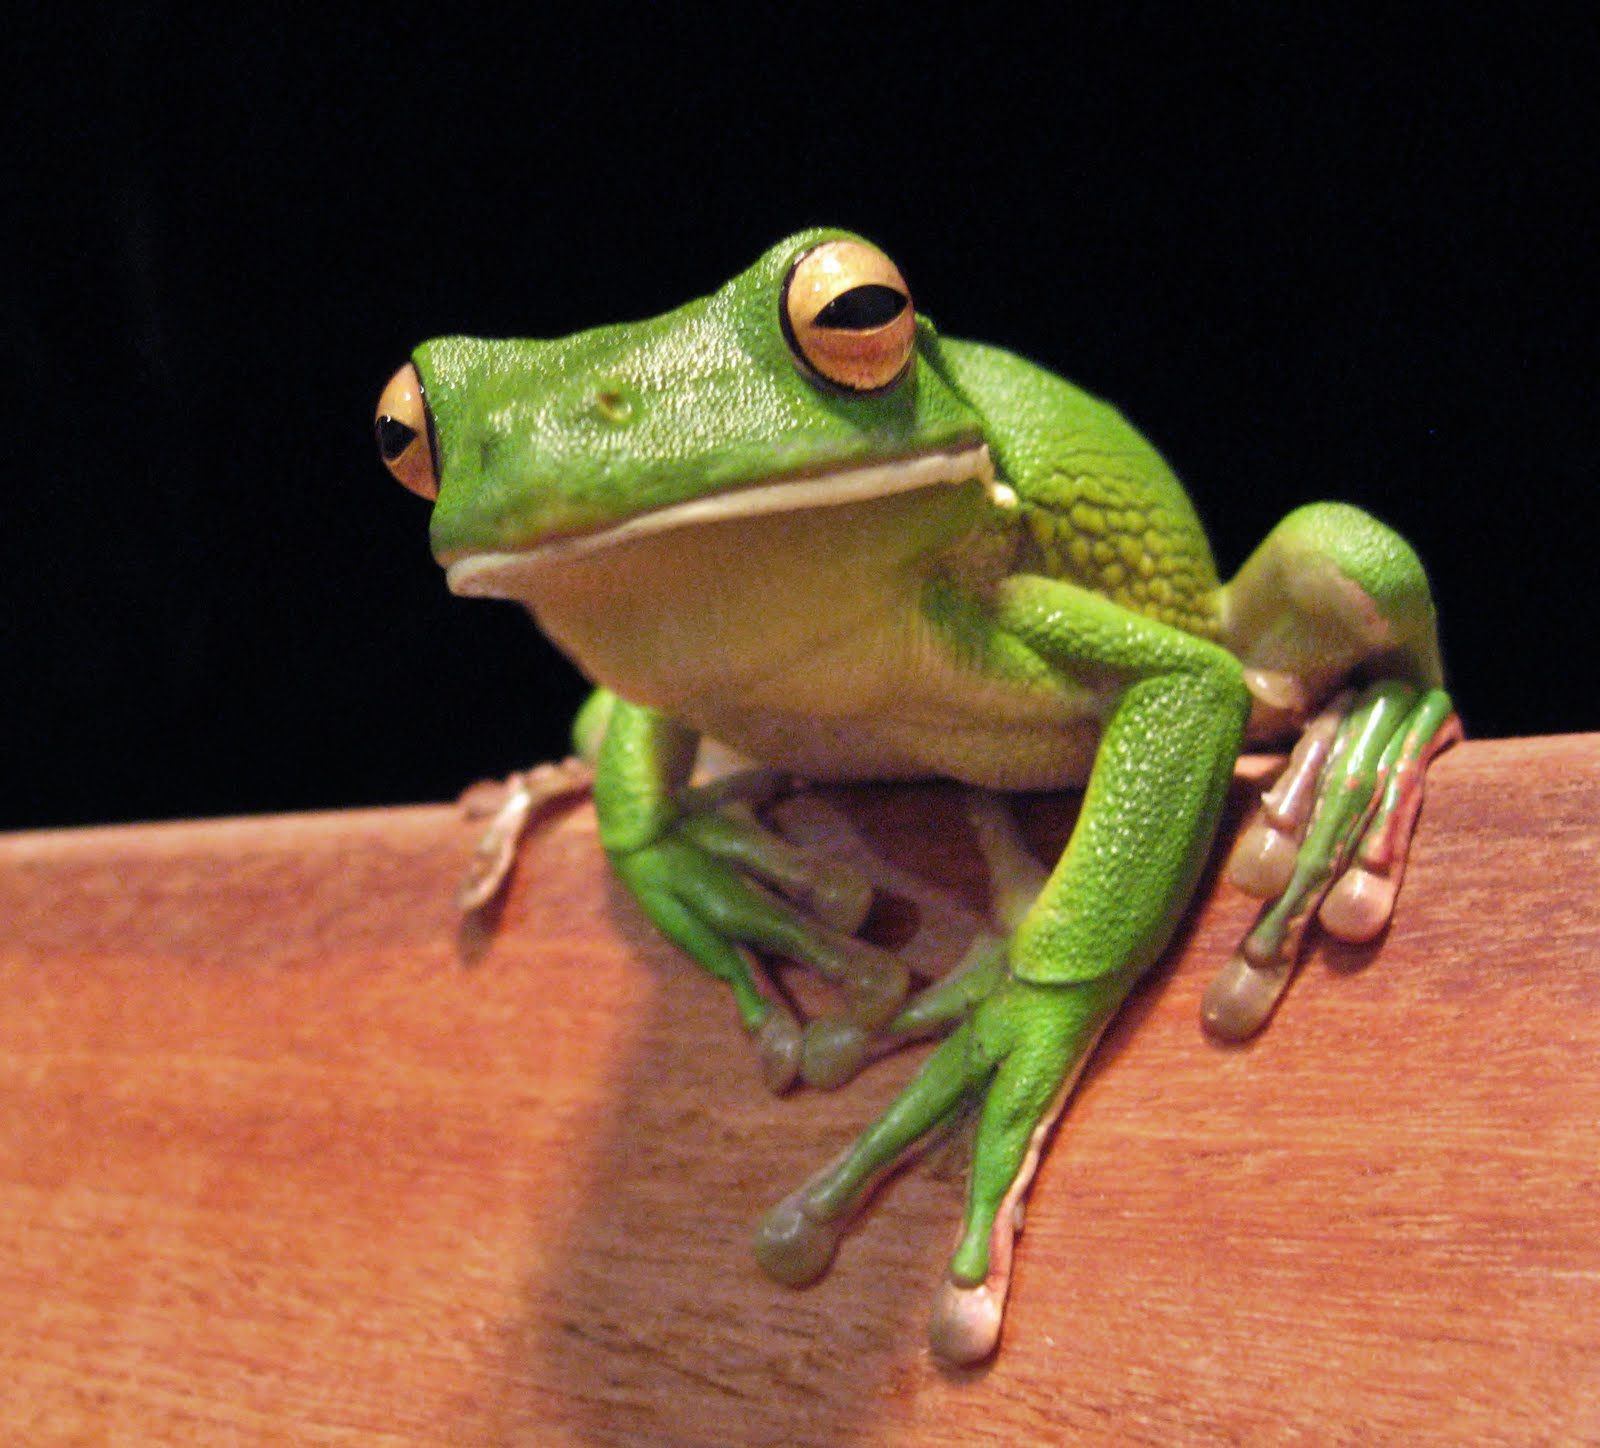
\includegraphics[width=0.25\linewidth]{frog.jpg}
	\caption{This is a figure}
	\label{fig:1}
\end{figure}

\begin{equation}
	x^2+y^2=z^2
	\label{eq:1}
\end{equation}
\begin{equation}
e^{\pi} = -1
\label{eq:2}
\end{equation}

The cleveref package allows you to:
\begin{itemize}
	\item prefix the type of the reference automatically: \cref{fig:1}
	\item reference with small and capital initial letters: \Cref{eq:1}, \cref{eq:1}.
	\item reference a range: \crefrange{eq:1}{eq:2}
	\item get the type of the reference: \namecref{fig:1}, \namecref{eq:1}
	\item get the page number of the reference: \cpageref{eq:1}
\end{itemize}

\end{document}